\chapter{METHODOLOGY}
\section{System Overview}
The automated hydroponic system is designed to maintain optimal nutrient solution chemistry and environmental conditions through continuous monitoring and closed-loop control. The system integrates high-accuracy sensors, an ESP32-based control unit, automated actuators, and cloud-based monitoring to regulate \gls{ph}, Total Dissolved Solids (\gls{tds}/Electrical Conductivity), and ambient humidity for hydroponic crop cultivation. The system is powered using a regular AC supply and provided with a battery backup in case of power outage.
\begin{figure}[H]
    \centering
    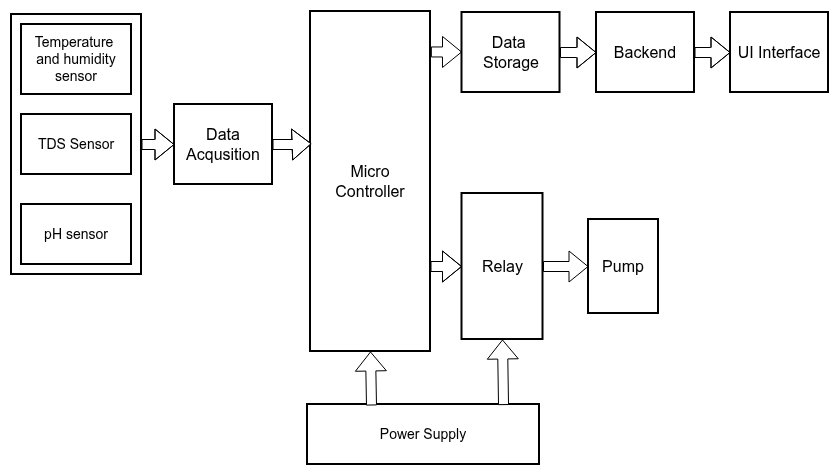
\includegraphics[width=1\linewidth]{src/images/blockDiagram.png}
    \caption{Block Diagram}
    \label{fig: Block_Diagram}
\end{figure}

\section{Sensor Subsystem}
The sensing subsystem is responsible for real-time acquisition of nutrient and environmental parameters:
\begin{itemize}
    \item \gls{ph} Measurement:\\
     An pH circuit paired with a probe (range 0–14 \gls{ph}) continuously measures the acidity/alkalinity of the nutrient solution. The pH sensor having power rating of 0.5W has input voltage of 3.3-5.5V and working current of 5-10mA. Its output voltage is 0-2.3V and the measurement range is 0-14. It has an accuracy of ±0.1pH and resolution of 0.01pH.
     \item TDS / Electrical Conductivity Measurement:\\
     A TDS sensor measures nutrient concentration by converting electrical conductivity into ppm values. Temperature compensation is applied using ambient temperature data to improve accuracy. The TDS sensor has input voltage of 3.3-5.5V and working current of 3-6mA. Its output voltage is 0-2.3V  and the measurement range is 0-1000 ppm. It has an accuracy of ±2.5\% and resolution of 1ppm.
     \item Humidity and Temperature Measurement:
     A DHT22 digital sensor module provides precise relative humidity and temperature readings through a wire interface, enabling environmental regulation. The DHT22 sensor has input voltage of 3.3-6V and working current of 1.5-2.5mA. It gives digital output. It has an accuracy of ±0.5\% and resolution of 0.1 degree for temperature and accuracy 2-5\% \gls{rh} and resolution of 0.1\% \gls{rh} for humidity.    
\end{itemize}

\section{Control and Processing Unit}
An \gls{esp}32-WROOM-32 microcontroller acts as the central controller. Its operating voltage is 3.3V and the maximum current it can handle is 40mA. Its responsibilities include:
\begin{itemize}
    \item Processing sensor data via ADC and I$^2$C interfaces
    \item Executing closed-loop control algorithms
    \item Handling Wi-Fi communication for cloud logging and alerts
\end{itemize}
Crop-specific setpoints are stored in memory and can be updated remotely.
\begin{figure}[H]
    \centering
    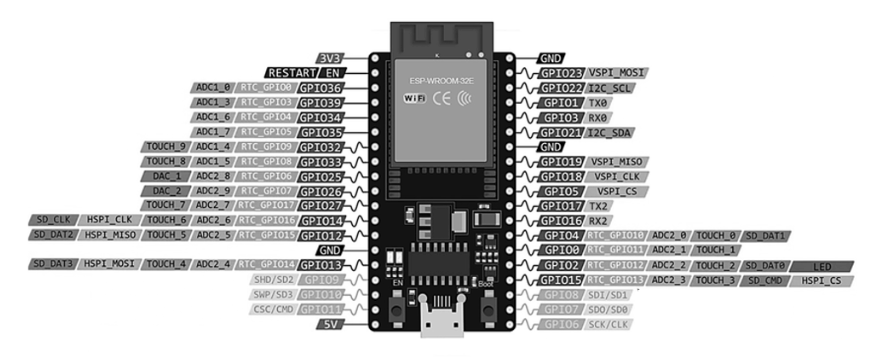
\includegraphics[width=1.04\linewidth]{src/images/ESP32.png}
    \caption{ESP32 pinout diagram}
    \label{fig:ESP32}
\end{figure}

\section{Actuation and Nutrient Control}
\subsection{TDS / EC Regulation}
\begin{itemize}
    \item If TDS is below the setpoint, macro and micro-nutrient solutions are dosed using pumps in a 3:1 ratio.
    \item EC correction is always performed prior to pH adjustment to avoid interaction effects.
\end{itemize}

\subsection{pH Regulation}
\begin{itemize}
    \item If measured pH exceeds the upper threshold, an acid dosing pump is activated.
    \item A 5-minute stabilization delay follows each dosing cycle before re-measurement.
\end{itemize}

\subsection{Humidity Control}
\begin{itemize}
    \item If relative humidity exceeds the setpoint, an exhaust fan is activated.
    \item Environmental control is temporarily paused during nutrient dosing to ensure measurement stability.
\end{itemize}

\section{User Interface and Data Logging}
\begin{itemize}
    \item The meter readings for pH, TDS, temperature and humidity sensors are transmitted via ESP-NOW protocol to a backend which are then displayed on a website. Device-to-device communication uses ESP-NOW with built-in encryption support, reducing the risk of unauthorized data access. The absence of direct internet exposure at the sensor node level further enhances system security.
    \item The website bridges the gap between human and machine as it enables users to monitor, analyze, and control system parameters efficiently. The website has simple UI/UX design which ensures the critical system information can be understood clearly. Sensor readings and system logs are stored in a Supabase database, which provides a cloud-based, scalable backend for secure data storage and historical data analysis.
    \item A dashboard based layout is used to display real time sensor parameters such as pH, EC, temperature, and humidity through visual cards. It also provides control over parameter setpoints i.e sensor threshold values, pump switch ON/OFF time, and exhaust fan switch ON/OFF time. Overall, the UI/UX design enhances user interaction with the hydroponic system. The calibration inputs are taken from the user and the user is provided with a datasheet including setpoints for each specific crop.
\end{itemize}

\section{Other Hardware Components}
\subsection{Relay Module}
A relay module is an electrically operated switch that allows low-voltage control signals from the microcontroller to switch high-voltage devices safely. It is used to control the operation of water pumps.

\begin{itemize}
\item Input Voltage: 5V DC  
\item Output Voltage: Up to 220V AC / 30V DC  
\item Current Rating: 10A
\end{itemize}

\subsection{Submersible Pump}
The submersible pump is used to circulate water from the reservoir to the plant growing channels. It operates fully immersed in water and ensures continuous water flow.
\begin{itemize}
\item Input Voltage: 220–240V AC 
\item Current Rating: 100 - 120 mA   
\item Power Rating: 25W
\end{itemize}

\subsection{5V DC Pump}
The 5V DC pump is employed for controlled liquid transfer in small-volume applications such as nutrient dosing and pH balancer.
\begin{itemize}
\item Input Voltage: 5V DC 
\item Current Rating: 130 - 220 mA  
\item Power Rating: 2.5W
\end{itemize}

\subsection{Regulated AC Power Adapter (12V DC / 2A)}
This adapter converts AC mains power into regulated 12V DC required for powering pumps and voltage regulation modules.
\begin{itemize}
\item Input Voltage: 220–240V AC  
\item Output Voltage: 12V DC  
\item Current Rating: 2A  
\item Power Rating: 24W
\end{itemize}

\subsection{3.3V to 5V Logic Level Shifter}
The logic level shifter enables safe bidirectional voltage translation between 3.3V and 5V logic signals, allowing communication between the microcontroller and peripheral modules.
\begin{itemize}
\item Input Voltage: 3.3V / 5V \gls{dc}  
\item Output Voltage: 5V / 3.3V DC  
\item Current Rating: Up to 50 mA per channel  
\item Power Rating: Less than 0.25W
\end{itemize}

\subsection{LM2596 Buck Converter}
The LM2596 is a step-down (buck) DC–DC converter used to efficiently reduce higher DC voltages to stable lower voltages required by sensors and control circuits.
\begin{itemize}
\item Input Voltage: 4–40V DC  
\item Output Voltage: 1.25–35V DC (Adjustable)  
\item Current Rating: Up to 3A  
\item Power Rating: Up to 45W
\end{itemize}

\subsection{DC Fan}
The DC Fan is used as an exhaust to the system.
\begin{itemize}
\item Input Voltage: 12V DC
\item Current Rating: 0.8 A
\item Power Rating: 9.6W
\end{itemize}

\section{Safety, Reliability, and Fail-Safes}
\begin{itemize}
    \item Maximum pump runtime limits prevent overdosing.
    \item Sensor fault detection halts the system and triggers alerts.
    \item Battery backup ensures data integrity during power outages.
    \item Antifouling measures and periodic probe cleaning enhance long-term reliability.
\end{itemize}
\section{Overall Working Principle}
The system operates continuously in a closed-loop feedback manner, prioritizing EC control, followed by pH and humidity regulation. Automated calibration, safety mechanisms, and cloud-based monitoring ensure stable long-term operation, minimal human intervention, and optimal crop growth conditions.
\subsection{Experimental Crop}
For our hydroponics system, we are experimenting with leafy green vegetables, specifically lettuce (Lactuca sativa) for the validation of the system. Lettuce is a suitable crop for hydroponic cultivation as it has a short growth cycle, comparatively low nutrient demand, and sensitive to parameter variations in the nutrient solution such as pH and EC. Additionally, the common growth cycle of 1 to 1.5 months creates opportunities for multiple experimental periods within the limited timeframe provided. These mentioned features of lettuce make it an ideal experimental crop for evaluation of the stability and effectiveness of the automated nutrient dosing control system.\\[10pt]
As lettuce is already a specialized crop in the hydroponics system, the growing conditions in manual hydroponics are well-documented in existing studies, allowing contrast and comparison between the experimental results and the standard results.

\subsection{Experimental Protocol}
The experimental procedure of the proposed system is to be performed using an automated hydroponic setup which operates over a crop growth cycle of lettuce (Lactuca sativa). This system consists of a closed-loop automated control of pH and EC based on the predefined setpoints provided for the leafy vegetables.\\[10pt]
Firstly, seedlings will be introduced to the automated hydroponic system for transplantation. During the experimental period, the system will monitor the nutrient solution parameters in the interval of 10 minutes and autonomously react through corrective dosing as per the deviation from the specified range of pH and EC. Furthermore, stabilization delays will be applied after each dosing process to allow the nutrients to mix uniformly before the measurements are taken. During each dosing event, the system introduces a priority-based control sequence where EC is balanced before adjusting pH. This is because the concentration of nutrients in the solution influences the acidity of the solution. Conventional IoT-based hydroponic systems generally enforce immediate threshold-triggered nutrient dosing, where corrective dosing is applied as soon as parameter deviations are detected. Such approaches often neglect the inherent mixing delay of nutrient solutions, which can result in overshoot. To overcome such limitations, the proposed system implements a stabilization-aware threshold based closed-loop control strategy. Instead of applying a classical PID control, the system utilizes a threshold-based proportional dosing mechanism. This control strategy is particularly suited for low-cost embedded platforms and hydroponic systems characterized by slow dynamic response, where robustness and stability are prioritized over aggressive control action.\\[10pt]
During the experimental period, readings from sensors, dosing events, and nutrient consumption data will be monitored and recorded.The collected results then will be compared to the reference data published in reports related to manual hydroponics system cultivating similar crops i.e. lettuce on the basis of parameters such as nutrient consumption, crop yield, pH and EC stability. Benchmark values for pH variation, EC fluctuation, nutrient consumption, and crop growth indicators will be extracted from peer-reviewed studies and technical reports.
\begin{table}[H]
\centering
\caption{Comparison of Timer-Based, PID-Based and Proposed Control Systems}
\label{tab:Comparison}
\renewcommand{\arraystretch}{1.4}
\begin{tabularx}{\textwidth}{|
>{\arraybackslash}L|
>{\arraybackslash}X|
>{\arraybackslash}X|
>{\arraybackslash}X|
>{\arraybackslash}X|}
\hline
\textbf{S.N.} & \textbf{Feature} & \textbf{Timer-Based System} & \textbf{PID-Based System} & \textbf{Proposed Control System}\\
\hline
1 & Control logic & Fixed intervals & Continuous feedback & Threshold-based closed-loop \\
\hline
2 & Threshold-based closed-loop & Very low & High & Low \\
\hline
3 & Overshoot risk & High & Moderate & Low \\
\hline
4 & Sensor dependency & Low & High & Moderate \\
\hline
5 & Suitability for low-cost MCU & High & Low & Moderate \\
\hline
6 & Adaptability & Poor & High & Moderate \\
\hline
\end{tabularx}


\end{table}

\begin{figure}[H]
    \centering
    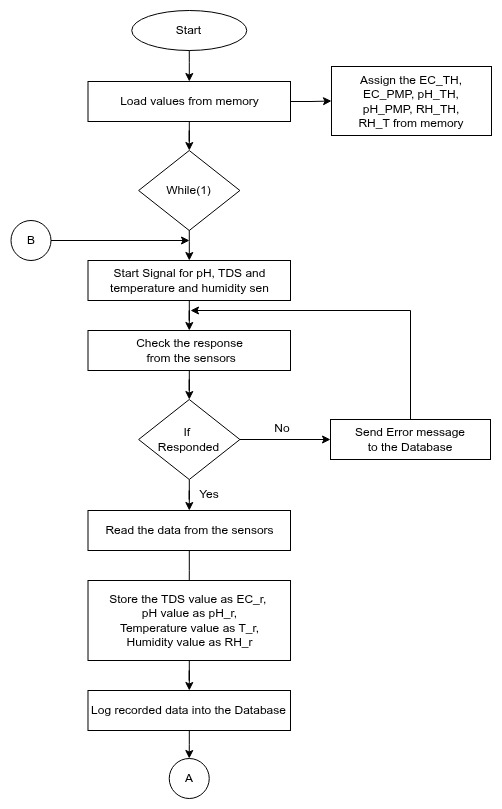
\includegraphics[width=1\linewidth]{src/images/Flowchart1.jpg}
\end{figure}
\begin{figure}[H]
    \centering
    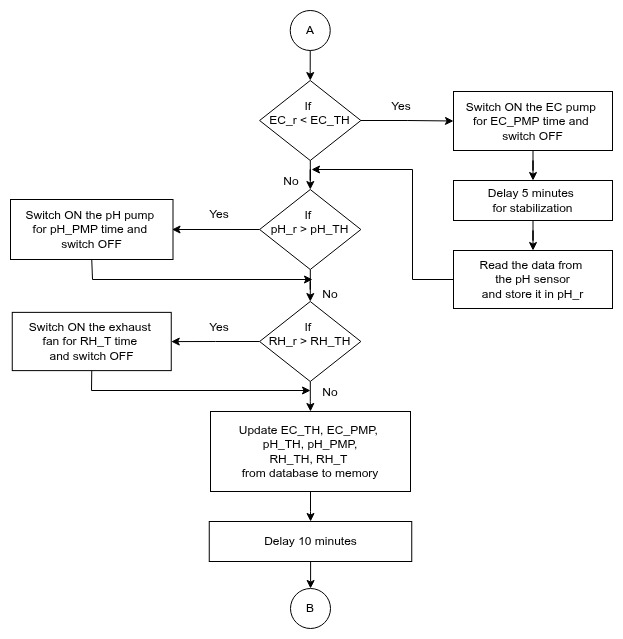
\includegraphics[width=1\linewidth]{src/images/Flowchart2.jpg}
    \caption{Flowchart}
    \label{fig:Flowchart}
\end{figure}